% !TEX root = comparison.tex
%% \section{Introduction} %for journal use above \firstsection{..} instead
%We introduce and discuss a tool for comparing different charts that are renderings of the same data in order to evaluate them for efficiency.
So, you've just spent countless hours burning the late night candle
wax and discovered several astonishing features in the data. Your
exploratory graphics are quick to produce, interactive, flexible, and
fabulous for discovery, but now you need to present the information to
your boss, the co-workers, a class of students, or get it published in
that top-rated journal. Those exploratory graphics are unlikely to
communicate the discovered information to your audience efficiently,
or elegantly.  To decide on the best way to present the specific
information there can be many types of plots to choose from. The
decision process is assisted by past experience, personal aesthetic
preferences, the characteristics of the audience, and a good working
knowledge of general perceptual strengths and weaknesses of particular
displays \citep{cleveland:1984,heer:2010}. Perceptual studies are
thinly spread for data visualization and will probably
only cover very broad perceptual principles, primarily because they
tend to be based solely on simulated data. In order to study
perceptual principles in a controlled experimental setting simulated
data is unavoidable. This provides principles that may not apply
closely enough to a specific analysis task.  Faced with design
decisions for a very specific task requires a closer level of
detail. Focus groups \citep{Mazza07} can find small problems with
designs and move us closer to a final handful of possible
designs. Usability studies and case studies
(e.g. \citet{Plaisant:2004}, \citet{Shneiderman:2006}) typically focus
on the use of particular software for solving data exploration tasks.
These approaches lack broad audience validity and
objectiveness. Several papers indicate continuing issues arising with,
and suggestions for improving, evaluation of information
visualizations
\citep{North:2006,Ellis:2006,Viegas:2006,Munzer:2009}. 

%determined from data graphics user studies such as \citet{cleveland:1984} and the large MTurk study in \citet{}. But it is hard to take these general principles and apply them to specific visual communication task, especially in an objective manner. 

%knowledge of perceptual strengths and weaknesses,  . But it is hard to make the final decision on the design in an objective manner. We can make this process less subjective by conducting user studies to evaluate competing designs of the same data, and measure designs for their efficiency by recording how accurately and quickly viewers can extract pieces of information. User studies for evaluating different designs has a long standing tradition. For  statistical graphics user studies have their origin in the (convenience) study on evaluating difficulty of a set of different visual tasks by \citet{cleveland:1984}, which has recently been replicated with similar results based on a large MTurk study by \citet{heer:2010}.

%% Di needs to work on the next few paragraphs, too.

Here we suggest a new approach using recent research on visual
inference \citep{buja:2009,wickham:2010}. In visual inference, real
data plots are considered to be test statistics, and these are
compared with plots of data generated from a null hypothesis using a
lineup. A lineup is similar to the police lineup, and this is where
the name comes from. The suspect (the plot of the real data) is placed
randomly in a field of plots of null data, and an impartial viewer is
asked to identify the plot that is the most different. If the viewer
identifies the suspect it lends statistical signficance to the
conclusion that the real data is not consistent with the null
data. Figure \ref{lineup} has an example of a lineup. Overlaid density
plots are used to display the distribution of two groups (blue, red)
of data. We are interested to know whether the real data has a
significant diffeerence between the centers of the two groups. Plot
numbered 13 contains the real data. Did you pick that one? In this
plot the blue group has a flat density whereas the density of red
group is more peaked and concentrated to the left of the blue.

\begin{figure}[htbp]
   \centering
   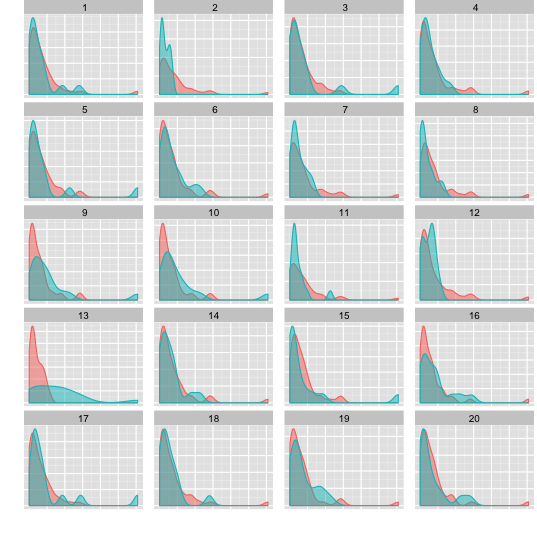
\includegraphics[height=0.95\linewidth]{density_1_45_15_20_13.png} 
   \caption{Example lineup using density plots: one plot of real data
     embedded with nineteen plots of null data. Which plot is
     most different from the others? (See the text for the answer.)}
   \label{lineup}
\end{figure}

The previous work \citet{buja:2009,wickham:2010} describes the use of
lineups for evaluating discoveries made in exploratory analysis. Here
we describe the use of lineups for evalating plot design for
communicating findings visually. Different lineups are created, using
the same data, same null plots and positions within the lineup, but
different plot designs. Comparing how long and how accurately the
viewers take to report the feature of interest will assess which
design is better for the task. To investigate the benefit of lineups
for plot design evaluation we have conducted an experiment that also
contains simulated data, where the data is constructed to match and
expand on the features of interest in the real data. For example, in a
simple situation, where the discovered feature of interest is a
difference between the centers of two distributions, simulated data
would be constructed roughly matching the distribution of the real
data that varies the distance between centers, and also spread and
sample size. Lineups of these simulated data (embedded with simulated
null data plots) are generated and evaluated along with the lineups of
real data. The simulation study provides a backdrop for the real data,
which enables the broad applicability to be studied and a gauge for
the signal strength of the pattern in the real data. 

%Usually, we need simulation studies to be able to completely control for the signal strength in the data. For charts, this is not a very realistic scenario. The need for displaying information particularly efficiently or accurately usually arises from  a particular problem while analyzing a data set, from which we want to learn new insight. Often, it is difficult to simulate data in such a way that it realistically represents the particular problem, which in turn makes it dubious whether the results from a simulation study are actually applicable to the problem at hand, reminding us painfully of George Box's famous quote on models: ``essentially, all models are wrong, but some are useful.'' \citep[page=424]{box}  

%Lineup \citep{buja:2009} allow us to directly use the data at hand to evaluate different competing designs by using permutations tests \cite{good:2011} of the original dataset. We can therefore get valid quantitative measures for comparing different designs without having to set up a simulation.

%When we are presenting a chart we  want to convince our audience of the presence of a particular feature or relationship in the data. In order to enable us to draw a conclusion about presence or absence of a feature in the data, we have, however, to assess what features show up based purely on marginal distributions rather than joint distributions.

%\begin{figure}[htbp] %  figure placement: here, top, bottom, or page
%   \centering
%   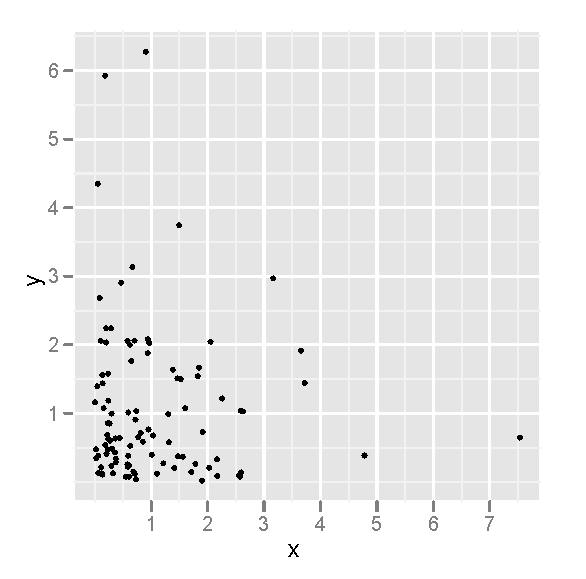
\includegraphics[height=0.32\linewidth]{rexp.pdf} 
%   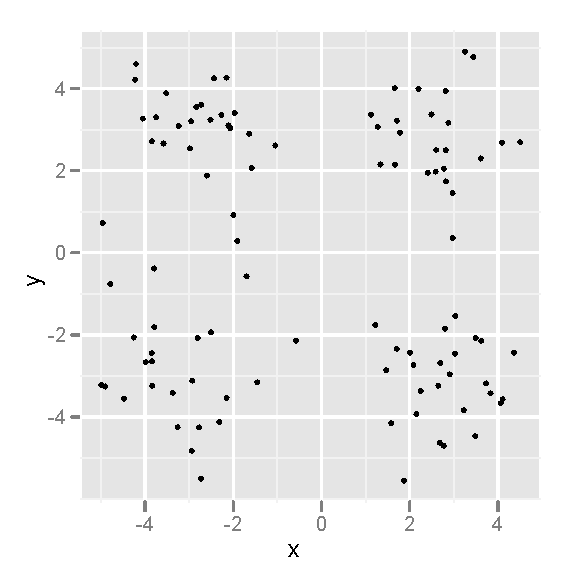
\includegraphics[height=0.32\linewidth]{rnorm.pdf} 
%   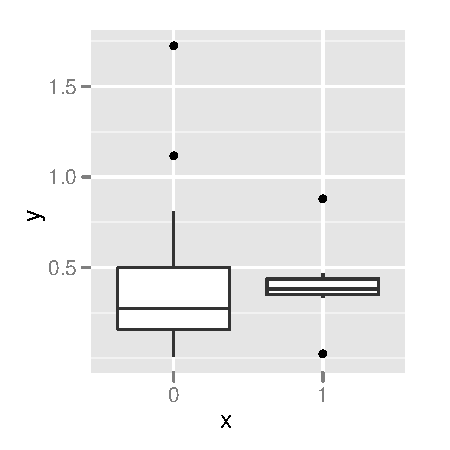
\includegraphics[height=0.32\linewidth]{two-exp.pdf} 
%   \caption{Examples of charts with distinctive features but independent variables. From left to right: scatterplot of $X$ and $Y$ with independent $X, Y \sim Exp_{\lambda=1}$; scatterplot of two variables with mixed normal distribution $N(3,1)$ and $N(-3,1)$; boxplot of $X$ and $Y$ with $X \sim B_{n=100, p=0.1}$ and $Y \sim Exp_{\lambda=1}$. }
%   \label{random}
%\end{figure}

%Features in the marginal distributions, such as multi-modality, skewness  or outliers, might interfere with our intuition of what `randomness' might mean in a particular situation and lead us to wrong conclusions. All of the plots in figure \ref{random} show distinctive features. None, of these, however, is a feature of the joint distribution, i.e. all of the variables involved are independent of each other. The scatterplot on the left of figure \ref{random} shows data sampled from an exponential distribution with rate parameter $\lambda=1$. The data in the middle comes from mixing two normal distributions with different means: half of the points has mean $\mu_1 = -3$, the other half has mean $\mu_2=3$, which results in the distinctive four groups. The two boxplots on the right appear to show a median shift between the two groups. This, however is a result of both the group size (only 7\% of the points is in the second group) and a skew distribution in vertical direction, with $y \sim Exp_{\lambda=1}$. 

%Lineup plots have been shown as an effective tool \cite{wickham:2010} for enabling us to quantitively assess the strength of the relationship between $X$ and $Y$. In a lineup plot the plot of the actual data is -- as in a police line-up -- inserted among decoy plots. The decoy or {\it null} plots are generated in a way that is consistent with the null hypothesis, i.e. these are plots in which we can assume that any relationship visible is there purely by chance. This gives us a reference framework against which to compare the data plot and, if we are still able to identify the data plot from the lineup because of a distinguishing feature, we have formal evidence that the feature in the data is, in fact, not just coincidental. 

Lineups provide a way to statistically quantify the significance of the finding
\citet{majumder:2011}. Think of the linup as a set of $m$ plots, one of which is the real data. For one lineup and one observer, the significance level, $\alpha$ is $1/m$. This is the probability that the observer picks the plot of the real data by chance. It is the probability of picking the real data plot, when it is really *not* different from the other null plots, that is a Type I error. (In Figure \ref{lineup}, $m=20$.) The power of a test is the probability that the real data plot is identified when it really is different from the null plots. Power is usually difficult to calculate because it is requires specific use of alternative hypothesis to calculate the probability.  Work in \citet{niladri:2012} addresses this to some extent with measures on the quality of a lineup, how different numerically, as best it can be calculated, the real data plot is from the null plots. 
%
When there are multiple observers the significance level also depends on the number of independent observers ($n$). Let $n$ be the number of independent observers and $x_i$ the number of observers who picked plot $i$, $i \in \{1, ..., m\}$, from the lineup. Then $(x_1, x_2, ..., x_m)$ follows a multinomial distribution Mult$_{\pi_1, \pi_2, ..., \pi_m}$ with $\sum_i \pi_i = 1$, where $\pi_i$ is the probability that plot $i$ is picked by an observer, which we can estimate as $\widehat{\pi_i} = x_i/n$. 

*** Under the null that the real is no different from the null, isn't $\pi_i=1/m$? Fixing this then I think the next paragraph on signal strength flows right from this one. It is when we are calculating signal strength that we start counting the number of observers who pick it.

%The power of a test is the probability to reject the null hypothesis, when it is not true. In the framework of lineups, power is, effectively, the probability that the data plot is identified. , i.e. power can be estimated as $x/n$, where $x$ is the number of observers who correctly identifies the plot of the real data out of $n$ observers.

%Let $x$ be the number of observers who
%correctly identify the plot of the real data. The probability that one
%observer correctly identifies the real data plot, in a size $m$
%lineup, by chance is $1/m$. 

\paragraph{Signal Strength}
To incorporate the results from multiple
observers think about the lineup as $m-1$ head-to-head competitions of
the data plot against $m-1$ null plots, which the data plot has to
win, is picked as the plot with the most distinct features. Assume
that the data plot is the one with the strongest signal, then the
probability that the data plot is picked by $x$ observers follows a
Beta distribution for the maximum \citet{****}:
\[
\text{signal strength} =  \left( \frac{x}{n}\right)^{1/(m-1)}.
\]
We call it signal strength \citet{majumder:2012}, and it is analogous to 1-$p$-value of a classical hypothesis test. Signal strength will range between 0 and 1, with higher values indicating stronger signal, more distinctive feature in the data.




The significance depends on the size ($m$) of
the lineup ($m=20$ in Figure \ref{lineup}) and the number of
independent observers ($n$). Let $x$ be the number of observers who
correctly identify the plot of the real data. The probability that one
observer correctly identifies the real data plot, in a size $m$
lineup, by chance is $1/m$. To incorporate the results from multiple
observers think about the lineup as $m-1$ head-to-head competitions of
the data plot against $m-1$ null plots, which the data plot has to
win, is picked as the plot with the most distinct features. Assume
that the data plot is the one with the strongest signal, then the
probability that the data plot is picked by $x$ observers follows a
Beta distribution for the maximum \citet{****}:
\[
\text{signal strength} =  \left( \frac{x}{n}\right)^{1/(m-1)}.
\]
We call it signal strength, and it is analgous to power in classical hypothesis testing. Signal strength will range between 0 and 1, with higher values indicating stronger signal, more distinctive feature in the data.

*** The above paragraph needs more explanation, and a reference for the beta distribution. I don't think the Majumder paper really is the source for this result is it? It leads up to it, but this is the new work that is not submitted yet.

*** Also need to refer to Niladri's ``Where's Waldo paper'' here too.

%The strength of this evidence is determined by both the number of independent evaluations as well as the size of the lineup. Assume a lineup of size $m$ is evaluated by $n$ independent observers, out of which $x$ identify the data plot correctly, which we can use as an estimate for the probability to correctly identify the data plot: this leads us to an estimate for the probability of correctly identifying the plot of $x/n$, with 95\% confidence intervals  for $x/n$ given as $x/n \pm 1.96 \cdot \sqrt{x/n \cdot (1-x/n)}$ limited to the interval [0,1]. Note, that the resulting interval is often too large to be useful.

%We can think of a lineup as $m-1$ head-to-head comparisons of the dataplot and $m-1$ nullplots, which the dataplot all has to `win', in order to be picked as the plot with the most distinct features. Assuming that observers identify the plot with the strongest signal, the probability that data plot is picked follows a Beta distribution for the maximum: this allows us to introduce the {\it signal strength} \cite{majumder:2011} of a lineup as:

%Signal strength is limited to a range of values between 0 and 1. Higher values indicate stronger signal. In the case of a parametric situation (i.e. the feature shown in the chart can be described in parametric form as a real-valued vector $\theta$ in the data), it can be shown \cite{majumder:2011} that the signal strength is strongly correlated to the $p$-value of the corresponding statistical test for $\theta$.
 
Signal strength is used in our new work to evaluate the effectiveness of different plot designs. This paper describes two examples where we had real data analysis problems and decisions to make in order to communicate the results. Section \ref{designs} describes the process for comparing designs. Section \ref{setup} and describe the two data analysis problems and the experiments conducted to evaluate the plots designs. Section \ref{results} presents the findings of the experiments, and Section \ref{conclusions} presents conclusions and suggestions for future use.

\section{Comparison of Designs}\label{designs}
We are going to make use of the signal strength gained from multiple viewings of a lineup in order to evaluate competing designs as follows:
\begin{enumerate}
\item{{\bf Create Lineup Data:} create data for a lineup of size $m$ by  creating  $m-1$ permutations of $y$ or, in the case of a simulation study, drawing $m-1$ samples of size $n$ (the number of rows in the data) from the null distribution. Add the original data to the lineup data randomly between 1 and $m$. }
\item{{\bf Create lineups from competing designs:} using the same data, render lineups of all competing designs. }
\item{{\bf Evaluate Lineups:} by presenting the lineups to independent observers. Assess both signal strength and time needed by individuals to come to a decision. Note that each observer should only be exposed to each lineup data once.}
\item{{\bf Evaluate Competing Designs:} differences in signal strength or time to decision are due to differences in the design. In the case that individuals were shown multiple lineups (as part of a bigger study), it is possible to correct outcome measurements for an individual's visual ability. }
\end{enumerate}

XXXX should we include nullabor code?

The power of a statistical test is defined as the probability to reject the null hypothesis. Translated to the visual tests, power is the probability to identify the data plot from the lineup. 
Comparing power of competing designs therefore involves comparing percentages of correct responses $p_1$ and $p_2$. An $\alpha\cdot$100\% confidence interval for this comparison is given as 
\[
p_1 - p_2 \pm t_{1-\alpha/2, n-1} \sqrt{p_1(1-p_1)/n_1 + p_2(1-p_2)/n_2},
\]
where $n$ is the Welch-Satterthwaite \cite{welch:1947} estimate of the degrees of freedom. Note that we use $p_i = (x_i+1)/(n_i+1)$ and $n_i+2$ for a better coverage of the confidence interval \cite{agresti:1998}.

While this allows a direct comparison of the designs, we cannot adjust for the individuals' perceptual abilities.
In the case that we have multiple responses from each person (i.e. data is collected on several {\it different} lineup tasks), we can estimate for their perceptual ability and correct power differences between competing designs accordingly, e.g. by modeling power using  a subject-specific random intercept in a generalized linear model.




%We also know that humans learn about new information through a visual search pattern that emphasizes new information (Wolfe, 2002; Rensick, et al., 1997). Of course, the type of visualization should take the natural human inclinations into account as well. For instance, a good visualization will account for both the �gestalt? like perceptual tendencies as well as the detail-orientated nature of cognition (Kosslyn, Thompson and Ganis, 2002; Pylshyn,2003)



